\section{Wzór Viete'a}

% https://en.wikipedia.org/wiki/Vi%C3%A8te%27s_formula

Viete wyprowadził swoją formułę na $\pi$ obserwując stosunek pola $2^n$-kata foremnego do pola $2^{n+1}$-kata foremnego. Poprzez zwiększanie $n$ w nieskończoność, jesteśmy w stanie dostać stosunek $2^2$-kąta foremnego, czyli kwadratu, do pola koła w które został on wpisany. Można ją też wyprowadzić za pomocą tożsamości udowodnionej przez Eulera ponad 100 lat po śmierci Viete'a.

Wzór zaproponowany przez Viete'a, uznawany za prekursor analizy matematycznej w matematyce poprzez pierwsze wykorzystanie nieskończonego ilorazu, jest następujący:
\begin{equation}
    {2\over\pi}=\prod\limits_{k=1}^n{a_k\over2},
\end{equation}
gdzie $a_1=\sqrt2$ oraz
$$a_k=\sqrt{2+a_{n-1}}.$$

Wiemy, że
$${\sin x\over x}=\cos\frac x2\cos\frac x4...=\lim_{n\to\infty}\prod\limits_{k=1}^n\cos{x\over 2^n}$$
oraz
$$\cos\frac x2=\sqrt{{1+\cos x\over 2}}.$$
Jeśli wstawimy $x=\frac\pi2$ i oznaczymy $b_k=\cos{x\over 2^k}$, $b_1={\sqrt2\over2}$,  dostaniemy
\begin{align*}
    {\sin\frac\pi2\over\frac\pi2}&=\frac2\pi=\lim_{n\to\infty}\prod\limits_{k=1}^n\cos{x\over 2^2}=\lim_{n\to\infty}\prod\limits_{k=1}^nb_k=\lim_{n\to\infty}\prod\limits_{k=1}^n{a_k\over 2},
\end{align*}
gdzie 
$$a_k=2b_k=2\sqrt{{1+b_{k-1}\over 2}}=\sqrt{2+2b_{k-1}}=\sqrt{2+a_{k-1}}$$
i $a_1=\sqrt2$.

\subsection{Wyniki}

Na Wykresie~\ref{viete-error}. zaprezentowany jest wykres zbieżności algorytmu Viete'a. Eksperymentalne wyznaczenie rzędu zbieżności, tak jak i gradient prezentowanego wykresu, sugerują liniową zbieżność tej metody wyliczania Viete. Od około 8750 iteracji wartość zwracana przez metodę Viete'a pokrywa się z wartością biblioteczną.

\begin{figure}[!h]\centering
    \renewcommand{\figurename}{Wykres}
    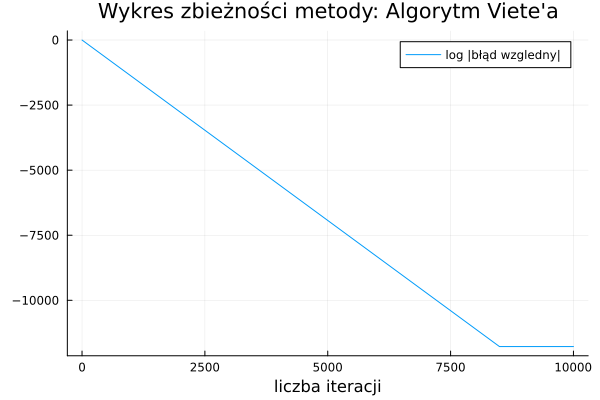
\includegraphics[width=0.7\textwidth]{../prog/viete_log_error.png}
    \caption{Wykres logarytmu dziesiętnego z błędu względnego dla przybliżenia $\pi$ za pomocą metody Viete'a.}
    \label{viete-error}
\end{figure}

\begin{figure}[!h]\centering
    \renewcommand{\figurename}{Wykres}
    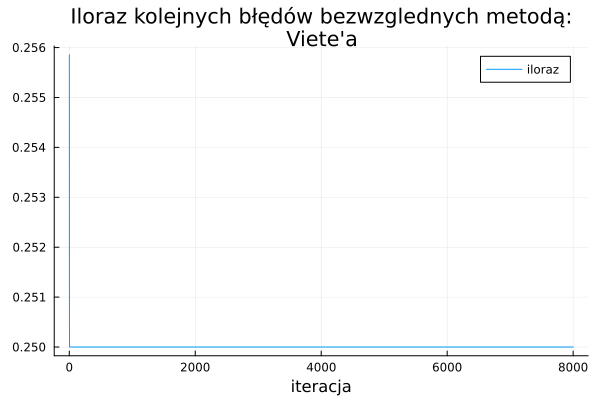
\includegraphics[width=0.7\textwidth]{../prog/viete_error_ratio.png}
    \caption{Wykres ilorazu błędów względnych wyrazu $n+1$ i $n$ dla metody z wykorzystaniem metody Viete'a.}
    \label{viete-convergence}
\end{figure}

Metoda Viete'a daje wyniki podobne do podejścia geometrycznego opisanego w Sekcji~\ref{geometric-interpretation}. Obie metody mają błąd bardzo bliski zera dla około 8000 iteracji metody. W obu metodach korzystamy z dwóch zmiennych, więc są podobne pamięciowo. W metodzie zaproponowanej przez Archimedesa musimy zapamiętywać obwód figury opisanej i wpisanej w okrąg, natomiast dla metody Viete'a potrzebujemy zapisywać dotychczasowy iloczyn oraz kolejny wyraz ciągu $a_k$. Różnią się one jedynie ilością operacji jakie wykonujemy w jednej iteracji, więc metoda Viete'a ma marginalnie lepszą stałą czasową.

Dodatkowo, jak widać na Wykresie~\ref{viete-convergence}., eksperymentalnie potwierdziliśmy, że metoda ta jest zbieżna liniowo. Tak jak w przypadku metody Archimedesa mamy
$$\lim_{k\to \infty}{|x_{k+1}-\pi|\over |x_k-\pi|}\approx\frac1{4},$$
gdzie $x_k$ to wynik $k$-tej iteracji metody.